\chapter{Metody algorytmiczne}\label{chap:algorithms}

W tym rozdziale przedstawiono wszystkie algorytmy zastosowane w pracy. Każdy algorytm opisano wraz z jego główną ideą, parametrami oraz analizą złożoności obliczeniowej.


Algorytmy zastosowane w pracy można podzielić na trzy grupy:
\begin{enumerate}
  \item \textbf{Metody dokładne} -- gwarantują znalezienie optymalnego rozwiązania: algorytm naiwny i programowanie całkowitoliczbowe (ILP).
  \item \textbf{Heurystyki konstrukcyjne} -- szybkie metody budujące rozwiązanie krok po kroku: algorytm zachłanny, zbiór dominujący, algorytm losowy.
  \item \textbf{Metaheurystyki} -- zaawansowane metody przeszukujące przestrzeń rozwiązań: algorytm genetyczny, przeszukiwanie tabu, algorytm mrówkowy, symulowane wyżarzanie.
\end{enumerate}

\section{Metody dokładne}

\subsection{Algorytm naiwny}\label{subsec:naive}
Algorytm naiwny jest metodą dokładną. Przegląda wszystkie podziały zbioru wierzchołków na dopuszczalne grupy oraz wszystkie przypisania licencji. Wybierane jest rozwiązanie o najniższym koszcie. Liczba rozważanych konfiguracji rośnie wykładniczo, dlatego metoda ma znaczenie praktyczne tylko dla bardzo małych instancji.

Na rysunku \ref{fig:all_types_time} przedstawiono czasy obliczeń w funkcji liczby wierzchołków dla grafów losowych, małoświatowych i bezskalowych. Do 12 wierzchołków czas wykonania pozostaje akceptowalny dla celów eksperymentalnych. Z uwagi na wykładniczy wzrost czasu działania algorytmu metoda ta staje się niepraktyczna dla większych instancji, zwłaszcza w kontekście dostępności bardziej efektywnych algorytmów, takich jak programowanie całkowitoliczbowe (ILP).

\begin{figure}[H]
  \centering
  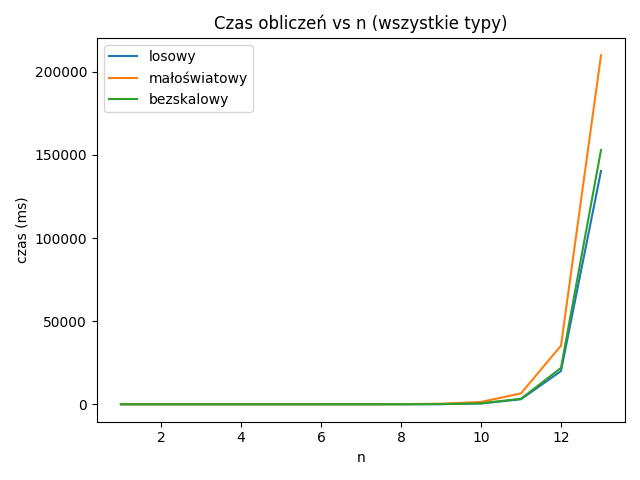
\includegraphics[width=0.66\textwidth]{assets/all_types_plot.png}
  \caption{Czas obliczeń algorytmu naiwnego w funkcji liczby wierzchołków $n$ dla trzech typów grafów}
  \label{fig:all_types_time}
\end{figure}

\paragraph{Idea metody}
\begin{enumerate}
  \item Wygenerować wszystkie partycje zbioru \(V\) na niepuste bloki (każdy blok odpowiada kandydatowi na grupę licencyjną).
  \item Dla każdego bloku w danej partycji wypisać wszystkie dopuszczalne pary (właściciel, licencja), czyli takie, które spełniają ograniczenia pojemności oraz sąsiedztwa.
  \item Łączyć wybory z poszczególnych bloków w pełne przypisania i odrzucać te, które nie pokrywają wierzchołków lub łamią ograniczenia.
  \item Obliczyć koszt na podstawie funkcji kosztu $\cost(f)$ (\ref{eq:cost_function}) i zapamiętać najlepsze rozwiązanie.
\end{enumerate}

\begin{algorithm}[H]
  \caption{Algorytm naiwny: pełny przegląd rozwiązań}
  \label{alg:naive}
  \begin{algorithmic}[1]
    \Require graf \(G=(V,E)\), zbiory licencji \( L\)
    \If{\(|V|>12\)} \State \Return przerwanie z powodu ograniczenia eksperymentalnego \EndIf
    \State \(best\_cost \gets \infty\), \(best \gets \emptyset\)
    \For{każda partycja \(P=\{P_1,\dots,P_k\}\) zbioru \(V\)}
    \For{każde przypisanie \(l\in L\) i właściciela w każdym \(P_i\)}
    \If{spełnione pojemności, sąsiedztwo i pełne pokrycie}
    \State policz koszt; zaktualizuj \(best\), jeśli lepszy
    \EndIf
    \EndFor
    \EndFor
    \State \Return \(best\)
  \end{algorithmic}
\end{algorithm}

\paragraph{Złożoność}
Algorytm generuje wszystkie partycje zbioru \(V\) na niepuste bloki, czyli wszystkie rozbicia odpowiadające potencjalnym zestawom grup licencyjnych. Takich partycji jest \(B_{|V|}\), gdzie \(B_m\) oznacza liczbę Bella dla \(m\) elementów. W implementacji nie ograniczamy z góry liczby bloków: niektóre typy licencji mogą pozostać nieużyte, dlatego dopuszczamy zarówno rozbicia na jedną grupę, jak i na \(|V|\) grup jednowskaźnikowych. Gdyby liczba bloków była stała i wynosiła \(k\), odpowiadałyby jej liczby Stirlinga drugiego rodzaju \({|V| \brace k}\); tutaj sumujemy je po wszystkich \(k\), stąd pojawiają się liczby Bella. Samo wygenerowanie partycji kosztuje więc $\Theta(B_{|V|})$.

Dla partycji o \(k\) blokach rozpatrujemy każdą kombinację wyboru właściciela (co najwyżej \(|V|\) opcji na blok) i dopuszczalnego typu licencji (co najwyżej \(T\) opcji, gdzie \(T=|L|\)). W skrajnym przypadku prowadzi to do górnego oszacowania \((|V|\cdot T)^k\) konfiguracji dla pojedynczej partycji. Jeśli ograniczenia pojemnościowe nie redukują przestrzeni, całkowity koszt można oszacować przez \(O\bigl(B_{|V|} \cdot (|V|\cdot T)^{|V|}\bigr)\). Wzrost jest superwykładniczy, ponieważ \(B_m\) przybliżają \({m^{m}}/(e^{m}\sqrt{m})\) dla rosnącego \(m\). W praktyce ograniczenia licencyjne i warunek sąsiedztwa znacząco zmniejszają liczbę rozważanych konfiguracji, lecz nawet wtedy pełny przegląd jest użyteczny wyłącznie dla bardzo małych grafów (rzędu kilku do kilkunastu wierzchołków).

Liczby Bella można zapisać wzorami
\[
  B_n = \sum_{k=0}^{n} \left\{\!\!\begin{array}{c} n \ k \end{array}\!\!\right\}\quad\text{oraz}\quad B_n = \frac{1}{e}\sum_{k=0}^{\infty}\frac{k^{\,n}}{k!},
\]
a zliczają one wszystkie rozbiory zbioru na dowolną liczbę niepustych bloków (bloki są nierozróżnialne). Dla porównania liczba wszystkich podzbiorów zbioru \(n\)-elementowego wynosi jedynie \(2^n\), więc nawet tak uproszczone oszacowanie rośnie wolniej niż pełna liczba partycji.

\subsection{Programowanie całkowitoliczbowe (ILP)}\label{subsec:ilp}

Programowanie całkowitoliczbowe formułuje problem z rozdziału~\ref{sec:model-formal} jako zadanie 
minimalizacji kosztu przy ograniczeniach liniowych oraz binarnych zmiennych decyzyjnych. 
Model ten został opracowany w ramach niniejszej pracy.
Metoda jest dokładna i zwraca rozwiązanie optymalne, o ile solver zakończy działanie poprawnie.

\paragraph{Parametry i zmienne}
Posługujemy się schematem licencyjnym z wzoru~\eqref{eq:license_family}, omówionym w~rozdziale~\ref{sec:model-formal}, czyli
\(
  L = \{ l_t = (c_t, m_t, k_t) \mid t = 1,\dots,T \},
\)
gdzie \(c_t\) oznacza koszt, \(m_t\) minimalną, a \(k_t\) maksymalną liczbę użytkowników (razem z właścicielem) obsługiwanych przez licencję typu \(t\). Korzystamy z notacji \(N[i]=N(i)\cup\{i\}\) oznaczającej otoczenie sąsiedztwa wraz z właścicielem. Dla każdego wierzchołka \(i\in V\) i licencji \(t\in\{1,\dots,T\}\) definiujemy zmienne binarne:
\begin{itemize}
  \item \(a_{i,t}\in\{0,1\}\) -- zmienna przyjmuje wartość 1 dokładnie wtedy, gdy węzeł \(i\) kupuje licencję typu \(t\) i tym samym aktywuje dla niej grupę licencyjną. Wartość 0 oznacza, że licencja \(t\) nie jest używana przez \(i\).
  \item \(x_{i,j,t}\in\{0,1\}\) -- zmienna ma wartość 1, gdy użytkownik \(j\) korzysta z licencji \(t\) nabytej przez właściciela \(i\), czyli jest członkiem jego grupy. Wartość 0 oznacza brak takiego przypisania. Zmienne te definiujemy tylko dla \(j\in N[i]=N(i)\cup\{i\}\), aby wymusić sąsiedztwo członków z właścicielem.
\end{itemize}
Zmienna \(x_{i,j,t}=1\) odwzorowuje przypisanie odbiorcy \(j\) do właściciela \(i\), dzięki czemu zbiory \(I\), \(H\) oraz \(R\) z rozdziału~\ref{sec:model-formal} reprezentowane są bezpośrednio przez wartości zmiennych.

\paragraph{Model matematyczny}
Model zapisujemy następująco:
\begin{align}
  \min\quad & \sum_{i\in V}\sum_{t=1}^{T} c_t\, a_{i,t}                    
            &  & \text{funkcja celu: całkowity koszt licencji} \\[6pt]
  \text{pod warunkami:}\quad
            & \sum_{i\in N[j]}\sum_{t=1}^{T} x_{i,j,t} = 1                   
            &  & \forall j\in V \label{con:cover} \\[6pt]
            & m_t\, a_{i,t} \le \sum_{j\in N[i]} x_{i,j,t} \le k_t\, a_{i,t} 
            &  & \forall i\in V,\ t=1,\dots,T \label{con:capacity} \\[6pt]
            & x_{i,i,t} = a_{i,t}                                              
            &  & \forall i\in V,\ t=1,\dots,T \label{con:owner} \\[6pt]
            & \sum_{t=1}^{T} a_{i,t} \le 1                                     
            &  & \forall i\in V \label{con:one}
\end{align}

\noindent
Znaczenie ograniczeń:
\begin{itemize}
  \item Ograniczenie~\ref{con:cover}: każdy wierzchołek jest przypisany dokładnie do jednej licencji - indywidualnej albo grupowej.
  \item Ograniczenie~\ref{con:capacity}: liczba uczestników w grupie musi mieścić się między najmniejszą a największą wartością przewidzianą przez dany typ licencji.
  \item Ograniczenie~\ref{con:owner}: właściciel zawsze uczestniczy we własnej grupie.
  \item Ograniczenie~\ref{con:one}: jeden wierzchołek może być właścicielem co najwyżej jednej licencji.
\end{itemize}
Ograniczenia te pokrywają się z warunkami wykonalności z rozdziału~\ref{sec:model-formal}.

\paragraph{Złożoność i zastosowanie}
Liczba zmiennych wynosi \(O\bigl(|V|\,T\,(\Delta+1)\bigr)\), gdzie \(\Delta\) to maksymalny stopień grafu, ponieważ dla każdego właściciela i typu licencji rozważane są przypisania do jego sąsiadów oraz do niego samego. W gęstych sieciach rośnie również liczba ograniczeń, co wydłuża czas działania solvera. W pracy model ILP służy jako złoty standard jakości rozwiązań dla małych i średnich instancji oraz jako źródło górnych ograniczeń dla metod przybliżonych.

\paragraph{Implementacja}
Model zaimplementowano w Pythonie z użyciem biblioteki \texttt{PuLP} i solvera \texttt{CBC} (\texttt{pulp.PULP\_CBC\_CMD}). Wartości zmiennych binarnych interpretowane są progowo przy rekonstrukcji rozwiązania \((>0.5\) traktowane jako prawda\().\) Funkcja celu oraz ograniczenia odzwierciedlają dokładnie przedstawiony model, dzięki czemu rozwiązania ILP odpowiadają etykietowaniu \(f\) opisanym w rozdziale~\ref{sec:model-formal}.

\section{Heurystyki konstrukcyjne}

\subsection{Algorytm zachłanny}\label{subsec:greedy}

Algorytm zachłanny to szybka heurystyka, która buduje rozwiązanie krok po kroku, w każdym kroku wybierając lokalnie najlepszą opcję. Algorytm nie gwarantuje znalezienia optymalnego rozwiązania, ale jest bardzo szybki i daje zazwyczaj w miarę dobre wyniki.

\paragraph{Idea metody}
Algorytm działa według następującej strategii:
\begin{enumerate}
  \item Sortuje wierzchołki nierosnąco według liczby sąsiadów (stopnia wierzchołka).
  \item Dla każdego wierzchołka sprawdza, czy może być właścicielem grupy.
  \item Wybiera typ licencji i rozmiar grupy tak, aby zminimalizować stosunek kosztu do rozmiaru grupy.
  \item Dodaje członków do grupy wybierając wierzchołki o największej liczbie sąsiadów.
  \item Powtarza proces dla wszystkich niepokrytych wierzchołków.
\end{enumerate}

Algorytm nie ma parametrów do dostrajania. Wszystkie decyzje są podejmowane deterministycznie na podstawie struktury grafu i kosztów licencji, choć w przypadku wierzchołków o tym samym stopniu kolejność wyboru może wpływać na wynik końcowy.

Sortowanie według stopnia wierzchołka (liczby sąsiadów) sprawdza się dobrze w praktyce, ponieważ wierzchołki o wysokim stopniu mogą tworzyć większe, bardziej efektywne grupy licencyjne.

\begin{algorithm}[H]
  \caption{Algorytm zachłanny}
  \label{alg:greedy}
  \begin{algorithmic}[1]
    \Require graf $G=(V,E)$, typy licencji $ L$
    \State posortuj wierzchołki nierosnąco według stopnia
    \State $niepokryte \gets V$
    \For{każdy wierzchołek $v$ w posortowanej kolejności}
    \If{$v$ już pokryty} \textbf{continue} \EndIf
    \State znajdź dostępnych sąsiadów $v$ wśród niepokrytych
    \For{każdy typ licencji $l_t \in L$}
    \State oblicz efektywność: $koszt_{l_t} / rozmiar\_grupy$
    \EndFor
    \State wybierz licencję i członków grupy o najlepszej efektywności
    \State utwórz grupę z $v$ jako właścicielem
    \State usuń członków grupy z $niepokryte$
    \EndFor
    \State \Return utworzone grupy
  \end{algorithmic}
\end{algorithm}


\paragraph{Złożoność i zastosowanie}
Algorytm ma złożoność czasową $O(|V|\,T + |E|\log |V|)$, gdzie $|V|$ to liczba wierzchołków, $|E|$ to liczba krawędzi, a $T$ to liczba typów licencji.
Algorytm zachłanny jest bardzo szybki i daje stabilne wyniki. Z tego powodu często używany był jako:
\begin{itemize}
  \item podstawowa metoda do porównywania z innymi algorytmami,
  \item źródło rozwiązania początkowego dla bardziej zaawansowanych metod,
  \item szybka metoda dla dużych grafów, gdzie inne algorytmy są zbyt wolne.
\end{itemize}
Wadą algorytmu jest to, że podejmując lokalnie najlepsze decyzje, może przegapić lepsze rozwiązania globalne.
\subsection{Heurystyka zbioru dominującego}\label{subsec:ds}

Heurystyka korzysta z konstrukcji \emph{minimalnych względem inkluzji} zbiorów dominujących. Zbiór dominujący jest minimalny, gdy usunięcie dowolnego jego wierzchołka powoduje utratę własności dominowania \cite{haynes1998domination}. W kontekście licencjonowania dominatorem nazywa się wierzchołek wybrany do zbioru dominującego, który stanie się właścicielem grupy licencyjnej i pokryje siebie oraz swoich sąsiadów. Dla przejrzystości zapisu wprowadzamy zbiór $F$ oznaczający wierzchołki, które nie zostały jeszcze przypisane ani do zbioru dominującego, ani do żadnej grupy licencyjnej.

Wskaźnik wyboru kandydata opiera się na \(\mathrm{coverage}(v)\) oraz \(\min\_\mathrm{cpn}(v)\).
\begin{itemize}
  \item $U$ to zbiór wierzchołków jeszcze niepokrytych, który jest bezpośrednią kopią $V$ na początku działania algorytmu. W miarę tworzenia grup wierzchołki są usuwane z $U$.
  \item \(\mathrm{coverage}(v)=|N[v]\cap U|\) to liczba jeszcze niepokrytych węzłów, które może pokryć \(v\).
  \item \(\min\_\mathrm{cpn}(v)\) to minimalny koszt na węzeł dla \(v\), liczony po wszystkich licencjach i dopuszczalnych rozmiarach grupy:
        \[
          \min\_\mathrm{cpn}(v)=\min_{l_t\in L}\;\min_{s\in[m_t,\;\min\{k_t,\ \mathrm{coverage}(v)\}]}\ \frac{c_t}{s}.
        \]
        Interpretacja: wybieramy dla \(v\) najkorzystniejszą licencję i rozmiar grupy, które dają najniższy koszt jednostkowy.
\end{itemize}

\begin{algorithm}[H]
  \caption{Zbiór dominujący z budowaniem grup}\label{alg:ds}
  \begin{algorithmic}[1]
    \Require graf $G=(V,E)$, zbiory licencji $ L$
    \State $U\gets V$, $D\gets\emptyset$, $R\gets V$
    \While{$U\neq\emptyset$}
    \State dla każdego $v\in V$ policz $\mathrm{coverage}(v)=|(N[v]\cap U|$ oraz $\min\_\mathrm{cpn}(v)$
    \State wybierz $u$ maksymalizujące $\mathrm{coverage}(v)/\min\_\mathrm{cpn}(v)$; jeśli brak rozstrzygnięcia wybierz dowolne $u\in U$
    \State $D\gets D\cup\{u\}$, $U\gets U\setminus N[u]$
    \EndWhile
    \State posortuj $D$ nierosnąco według stopni wierzchołków
    \For{każde $u\in D$}
    \State $S\gets N[u]\cap F$
    \State wybierz najtańszą dopuszczalną licencję dla $u$ i wyznacz grupę $P\subseteq S$ o największym dopuszczalnym rozmiarze; w ostateczności przydziel licencję indywidualną
    \State $F\gets F\setminus P$
    \EndFor
    \State \Return utworzone grupy
  \end{algorithmic}
\end{algorithm}

\paragraph{Złożoność i zastosowanie}
Faza wyboru dominatorów w każdej rundzie przechodzi po wszystkich wierzchołkach, ich sąsiadach i typach licencji, co daje koszt rzędu $O(|V||E|T)$. Faza budowania grup dla każdego dominatora sortuje kandydatów i sprawdza warianty licencji. W gęstych grafach rośnie to do \(O(|V|^3 T \log |V|)\), w rzadkich pozostaje bliżej $O(|V||E|T)$. Heurystyka w krótkim czasie wyznacza pełne pokrycie i dostarcza jakościowe rozwiązanie początkowe dla metod ulepszających.

\subsection{Algorytm losowy}\label{subsec:random}

Algorytm losowy pełni rolę metody odniesienia do oceny jakości rozwiązań generowanych przez inne algorytmy. Weryfikuje poprawność implementacji i stanowi stochastyczny punkt odniesienia. Wierzchołki są przetwarzane w losowej kolejności, a wybór licencji i składu grupy jest losowy w granicach ograniczeń pojemności i sąsiedztwa.

\paragraph{Idea metody}
\begin{enumerate}
  \item Losowana jest kolejność przetwarzania wierzchołków.
  \item Dla bieżącego wierzchołka wyznaczany jest zbiór kandydatów obejmujący jego oraz nieprzydzielonych sąsiadów.
  \item Jeżeli istnieje dopuszczalna licencja, losowany jest typ licencji, rozmiar grupy oraz członkowie grupy z dostępnych kandydatów.
        Rozważano wariant wyboru zgodnie z najlepszym kosztem jednostkowym \(\min_{l,s} c_l/s\), analogicznie do heurystyki zbioru dominującego.
        W tej pracy przyjęto jednak minimalną deterministyczność i maksymalną losowość do wyznaczenia górnego ograniczenia efektywności metaheurystyk.
  \item W przeciwnym razie przydzielana jest najtańsza dostępna licencja indywidualna.
  \item Kroki są powtarzane do pełnego pokrycia grafu.
\end{enumerate}

\paragraph{Uwagi o losowości}
Celem było uzyskanie szerokiego spektrum wyników, aby zobaczyć, jak zachowuje się heurystyka w losowych warunkach spełniających ograniczenia problemu.
Nie stosowano wariantu wyboru licencji według najlepszego kosztu na węzeł, ponieważ prowadziłoby to do wyniku deterministycznego i zawężenia rozkładu rezultatów. 
Rozważano także uruchamianie algorytmu wielokrotnie i wybieranie najlepszego otrzymanego wyniku spośród dużej liczby uruchomień.
Ze względu na dużą losowość w doborze licencji i składzie grup okazało się jednak, że średnia wartość jakości rozwiązania z wielu uruchomień nie różni się istotnie od wyniku pojedynczego najlepszego przebiegu.
Z tego powodu algorytm uruchamiany jest tylko raz z możliwością ustawienia ziarna generatora liczb losowych, co pozwala odtwarzać eksperymenty.

\begin{algorithm}[H]
  \caption{Losowy dobór licencji i składu grupy}\label{alg:randomized}
  \begin{algorithmic}[1]
    \Require graf $G=(V,E)$, zbiory licencji $ L$
    \State $U\gets V$, $\pi\gets$ losowa permutacja $V$
    \For{node w kolejności $\pi$}
    \If{$node\notin U$} \textbf{continue} \EndIf
    \State $S\gets N[node]\cap U$
    \If{istnieje licencja $l_t$ z $m_t\le |S|$}
    \State losuj $l_t$ oraz rozmiar $s\in\bigl[m_t,\min\{|S|,k_t\}\bigr]$, następnie losuj członków grupy z $S$
    \Comment{wariant kierowany: można zastąpić wyborem $\arg\min_{l_t,s} c_t/s$}
    \Else
    \State przydziel najtańszą licencję indywidualną
    \EndIf
    \State dodaj grupę, usuń jej członków z $U$
    \EndFor
    \While{$U\neq\emptyset$} przydziel najtańszą licencję indywidualną i usuń węzeł z $U$ \EndWhile
  \end{algorithmic}
\end{algorithm}

\paragraph{Złożoność i zastosowanie}
Każdy wierzchołek i jego sąsiedzi są przeglądani co najwyżej raz, a przy każdej próbie losowania licencji przeglądane są wszystkie typy licencji, co daje koszt rzędu \(O\bigl(T(|E|+|V|)\bigr)\).
W gęstych grafach upraszcza się to do \(O(T|V|^2)\).
Algorytm służy jako benchmark stochastyczny oraz kontrola jakości innych metod.
Wariant kierowany \(\min c_t/s\) nie zmienia rzędu złożoności i może być użyty pomocniczo do analizy wrażliwości.


\section{Metaheurystyki}

Metaheurystyki to zaawansowane algorytmy przeszukujące przestrzeń rozwiązań w sposób inteligentny. W przeciwieństwie do heurystyk konstrukcyjnych, które budują rozwiązanie od zera, metaheurystyki zaczynają od pewnego rozwiązania i systematycznie je poprawiają.

\paragraph{Dobór parametrów}
Parametry metaheurystyk zostały dobrane eksperymentalnie na podstawie testów na grafach różnych rozmiarów.

\paragraph{Operacje modyfikacji rozwiązania}
Metaheurystyki poprawiają rozwiązanie stosując następujące operacje:
\begin{itemize}
  \item zmiana typu licencji używanej przez właściciela grupy
  \item przeniesienie członka z jednej grupy do drugiej
  \item zamiana miejscami dwóch członków z różnych grup
  \item scalanie dwóch grup w jedną lub rozdzielanie na dwie dopuszczalne.
\end{itemize}

\subsection{Algorytm genetyczny}\label{subsec:ga}
Algorytm genetyczny utrzymuje populację pełnych przydziałów licencyjnych i z pokolenia na pokolenie ulepsza je, korzystając z losowych mutacji i krzyżowania par rodziców \cite{holland1975,goldberg1989}. Zaczyna od kilku rozwiązań zachłannych i losowych, a następnie w każdej generacji wybiera najlepsze osobniki (elita), losuje rodziców metodą turniejową i tworzy potomstwo przez krzyżowanie lub mutację. Słabsze rozwiązania są stopniowo zastępowane lepszymi, a algorytm zapamiętuje najlepszy znaleziony koszt.

\paragraph{Parametry}
\begin{itemize}
  \item \textbf{Wielkość populacji} $P=30$ - liczba rozwiązań utrzymywanych w każdej generacji.
  \item \textbf{Liczba pokoleń} $G=40$ - maksymalna liczba iteracji ewolucji.
  \item \textbf{Udział elity} $\alpha=20\%$ - część najlepszych osobników kopiowana bez zmian do kolejnego pokolenia.
  \item \textbf{Prawdopodobieństwo krzyżowania} $p_c=60\%$ - przy tej szansie dziecko powstaje przez połączenie dwóch rodziców; w przeciwnym razie wykonywana jest mutacja.
\end{itemize}

\begin{algorithm}[H]
  \caption{Algorytm genetyczny}
  \label{alg:ga}
  \begin{algorithmic}[1]
    \Require graf $G=(V,E)$, typy licencji $ L$
    \State utwórz populację początkową (zachłanny + losowe rozwiązania)
    \For{każde pokolenie}
    \State oceń wszystkie rozwiązania (funkcja kosztu)
    \State zachowaj elitę (najlepsze rozwiązania)
    \While{populacja niepełna}
    \If{losowanie krzyżowania}
    \State wybierz dwóch rodziców (selekcja turniejowa)
    \State skrzyżuj rodziców (połącz efektywne grupy)
    \Else
    \State wybierz rozwiązanie i zmutuj (operacje sąsiedztwa)
    \EndIf
    \State dodaj potomka do nowej populacji
    \EndWhile
    \State zaktualizuj najlepsze znalezione rozwiązanie
    \EndFor
    \State \Return najlepsze rozwiązanie
  \end{algorithmic}
\end{algorithm}

\paragraph{Złożoność i zastosowanie}
Inicjalizacja populacji korzysta z jednego osobnika otrzymanego za pomocą algorytmu zachłannego i $P-1$ losowych rozwiązań, co kosztuje około $O\bigl(P \cdot (|V|T + |E|\log |V|)\bigr)$. Każda generacja sortuje populację ($O(P\log P)$), a następnie tworzy nowe pokolenie. Mutacje wywołują ograniczoną liczbę operatorów sąsiedztwa (zmiana typu licencji, przeniesienie członka, zamiana miejscami, scalanie lub podział grup), a krzyżowanie w razie potrzeby uruchamia heurystykę zachłanną na podgrafie, co razem daje koszt rzędu $O(|V|T + |E|\log |V|)$ na potomka. Łącznie otrzymujemy $O\bigl(G \cdot P \cdot (|V|T + |E|\log |V|)\bigr)$ w najgorszym przypadku. Algorytm działa wolniej od prostych heurystyk, ale potrafi znacząco poprawić ich wyniki i służy jako główna metoda poszukiwania wysokiej jakości rozwiązań, gdy możemy poświęcić na optymalizację więcej czasu.


\subsection{Przeszukiwanie tabu}\label{subsec:tabu}
Algorytm tabu rozpoczyna działanie od rozwiązania uzyskanego heurystyką zachłanną, a następnie iteracyjnie przeszukuje lokalne sąsiedztwo. Sąsiadem nazywa się rozwiązanie otrzymane przez pojedynczą operację mutacji, na przykład zmianę typu licencji właściciela, przeniesienie członka między grupami, zamianę członków lub scalenie i podział grup. Lista tabu przechowuje podpisy ostatnich rozwiązań lub ruchów i zakazuje wyboru kandydatów, którzy prowadzą do niedawno odwiedzonych stanów. Kryterium aspiracji pozwala pominąć zakaz, gdy kandydat poprawia najlepszy dotąd koszt. Mechanizm ten ogranicza krótkie cykle i równoważy lokalne doskonalenie z eksploracją nowych przydziałów licencji \cite{glover1989}.

\paragraph{Parametry}
\begin{itemize}
  \item \textbf{Maksymalna liczba iteracji} \(I=1000\).
  \item \textbf{Długość listy tabu} \(L=20\) elementów.
  \item \textbf{Liczba sąsiadów na iterację} \(k=10\).
\end{itemize}

\begin{algorithm}[H]
  \caption{Przeszukiwanie tabu}\label{alg:tabu}
  \begin{algorithmic}[1]
    \Require graf \(G=(V,E)\), typy licencji \( L\)
    \State \(aktualne \gets\) rozwiązanie początkowe wyznaczone algorytmem zachłannym
    \State \(najlepsze \gets aktualne\)
    \State \(lista\_tabu \gets\) pusta kolejka o stałej długości \(L\); wstaw podpis \(aktualne\)
    \For{każdą iterację}
    \State wygeneruj sąsiedztwo \(aktualne\) przez operacje mutacji
    \State wybierz najlepszego kandydata, którego podpis nie znajduje się na \(lista\_tabu\) lub który poprawia \(najlepsze\) \((\)aspiracja\()\)
    \If{wybrano kandydata}
    \State \(aktualne \gets\) kandydat; zaktualizuj \(lista\_tabu\)
    \If{\(aktualne\) lepsze niż \(najlepsze\)} \State \(najlepsze \gets aktualne\) \EndIf
    \Else
    \State \textbf{break}
    \EndIf
    \EndFor
    \State \Return \(najlepsze\)
  \end{algorithmic}
\end{algorithm}

\paragraph{Złożoność i zastosowanie}
Inicjalizacja początkowego stanu grafu obejmuje jedno uruchomienie heurystyki zachłannej \(O(|V|T + |E|\log |V|)\). W każdej z \(I\) iteracji generowanych jest do \(k\) sąsiadów. Ocena kandydata obejmuje sprawdzenie pojemności, pokrycia i zgodności z sąsiedztwem w grafie, co kosztuje około \(O(|V|T + |E|)\). Łączna złożoność obliczeniowa wynosi w przybliżeniu \(O\!\left(I \cdot k \cdot (|V|T + |E|)\right)\). Przeszukiwanie tabu dobrze sprawdza się jako metoda ulepszająca: poprawia rozwiązania wyjściowe przy umiarkowanym czasie obliczeń i ogranicza powroty do niedawno odwiedzonych stanów dzięki liście tabu.

\subsection{Algorytm mrówkowy}\label{subsec:aco}
Algorytm mrówkowy buduje wiele rozwiązań równolegle. Każda mrówka konstruuje przydział licencji, kierując się siłą śladów feromonowych (informacja o dotychczas dobrych wyborach) oraz heurystyką preferującą wierzchołki o dużym stopniu i licencje o dobrym stosunku pojemności do ceny \cite{dorigo1997}. Po każdej iteracji, czyli po zakończeniu budowy rozwiązań przez wszystkie mrówki w danym kroku, feromony parują, a najlepsze dotąd rozwiązanie wzmacnia ścieżki feromonowe, czyli w przypadku naszej implementacji prawdopodobieństwo wyboru konkretnych właścicieli i typów licencji. 
Dzięki temu kolejne mrówki chętniej eksplorują obiecujące fragmenty przestrzeni rozwiązań (tj. wierzchołków i typów licencji).
\paragraph{Parametry}
\begin{itemize}
  \item \textbf{Waga feromonu} $\alpha=1.0$ -- określa, jak mocno mrówki ufają dotychczasowym śladom.
  \item \textbf{Waga heurystyki} $\beta=2.0$ -- wzmacnia lokalnie korzystne decyzje, czyli takie, które przy danym wierzchołku pozwalają dobrać licencję z wysoką pojemnością i niskim kosztem jednostkowym. Koszt jednostkowy to cena licencji $l_t$ podzielona przez liczbę użytkowników w grupie lub cenę licencji indywidualnej.
  \item \textbf{Tempo parowania} $\rho=0.5$ -- część feromonu usuwana po każdej iteracji.
  \item \textbf{Prawdopodobieństwo wyboru zachłannego} $q_0=0.9$ -- z tą szansą mrówka wybiera najlepszą dostępną opcję, w przeciwnym razie losuje wierchołek i licencje proporcjonalnie do wag wyliczonych w trakcie budowy rozwiązania.
  \item \textbf{Liczba mrówek} $A=20$ -- ile rozwiązań konstruujemy równolegle w jednej iteracji.
  \item \textbf{Maksymalna liczba iteracji} $I=100$ -- ile razy aktualizujemy feromony.
  \item \textbf{Losowe ziarno} (opcjonalne) -- pozwala odtworzyć przebieg eksperymentu.
\end{itemize}


\begin{algorithm}[H]
  \caption{Algorytm mrówkowy}
  \label{alg:aco}
  \begin{algorithmic}[1]
    \Require graf $G=(V,E)$, typy licencji $ L$
    \State zainicjalizuj feromony $\tau$ (dla par wierzchołek-licencja)
    \State zainicjalizuj heurystyki $\eta$ (na podstawie stopni wierzchołków i kosztów licencji)
    \State $najlepsze \gets$ rozwiązanie początkowe (zachłanne)
    \For{każdą iterację}
    \For{każdą mrówkę}
    \State $niepokryte \gets V$
    \While{$niepokryte \neq \emptyset$}
    \State wybierz właściciela na podstawie $\tau$ i $\eta$ (reguła wyboru lub ruletka)
    \State wybierz typ licencji na podstawie $\tau$ i $\eta$
    \State utwórz grupę, usuń członków z $niepokryte$
    \EndWhile
    \If{mrówka znalazła lepsze rozwiązanie}
    \State $najlepsze \gets$ rozwiązanie mrówki
    \EndIf
    \EndFor
    \State wyparuj część feromonów: $\tau \gets \tau \cdot (1-evaporation)$
    \State wzmocnij feromony na ścieżce $najlepsze$: $\tau \gets \tau + 1/koszt$
    \EndFor
    \State \Return $najlepsze$
  \end{algorithmic}
\end{algorithm}

\paragraph{Złożoność i zastosowanie}
Inicjalizacje feromonów i heurystyk charakteryzuje złożoność obliczeniowa $O(|V|T)$. Pojedyncza konstrukcja rozwiązania wymaga odwiedzenia przez mrówkę każdego wierzchołka co najwyżej raz. W każdym kroku mrówka wybiera wierzchołek, który stanie się właścicielem nowej grupy licencyjnej; w tym celu ocenia wszystkie niepokryte wierzchołki jako potencjalnych właścicieli oraz wszystkie typy licencji dostępne w zbiorze $L$. Po wskazaniu właściciela trzeba posortować jego sąsiadów w grafie $G$ według wag feromonowo-heurystycznych, aby zdecydować, którzy użytkownicy dołączą do grupy. Te operacje prowadzą do złożoności obliczeniowej rzędu $O(|V|^2 T + |E|\log |V|)$ na jedną mrówkę. Algorytm wykonujący $I$ iteracji z $A$ mrówkami ma więc złożoność $O\!\left(I \cdot A \cdot (|V|^2 T + |E|\log |V|)\right)$. Metoda jest bardziej złożona obliczeniowo niż tabu i algorytm zachłanny, ale pozwala eksplorować wiele alternatywnych konfiguracji i stopniowo wzmacniać najlepsze z nich.


\subsection{Symulowane wyżarzanie }\label{subsec:sa}
Symulowane wyżarzanie rozpoczyna od dowolnego dopuszczalnego przydziału; w implementacji korzystamy z rozwiązania wygenerowanego heurystyką zachłanną. W każdej iteracji losowana jest jedna z operacji modyfikacji opisanych na początku sekcji metaheurystyk. Jeżeli wylosowana operacja prowadzi do stanu naruszającego ograniczenia, losujemy kolejną do chwili znalezienia dopuszczalnego kandydata (maksymalnie kilkanaście prób na iterację). Nowy stan jest akceptowany zawsze, gdy obniża koszt całkowity przydziału licencji, a czasami także wtedy, gdy go pogarsza - z prawdopodobieństwem zależnym od bieżącej temperatury \(T\) i różnicy kosztów całkowitych rozwiązania bieżącego i kandydata \cite{kirkpatrick1983}. Temperatura maleje według ustalonego współczynnika, a gdy liczba kolejnych iteracji bez poprawy najlepszej wartości przekroczy limit stagnacji \(S\), jest dodatkowo dzielona przez dwa. Dzięki temu metoda potrafi opuszczać lokalne minima funkcji kosztu w sąsiedztwie zdefiniowanym przez powyższe operacje i stopniowo stabilizuje się w pobliżu dobrego rozwiązania.

\paragraph{Parametry}
\begin{itemize}
  \item \textbf{Temperatura początkowa} $T_0 = 100.0$ - stosunkowo wysoka wartość dobrana eksperymentalnie; przy takich temperaturach różnice kosztów rzędu kilku jednostek są często akceptowane, co pozwala na szeroką eksplorację przestrzeni rozwiązań na początku działania algorytmu.
  \item \textbf{Współczynnik chłodzenia} $\alpha = 0.995$ - w każdej iteracji temperatura jest mnożona przez $\alpha$.
  \item \textbf{Temperatura minimalna} $T_{\min} = 0.001$ - po jej osiągnięciu algorytm kończy działanie.
  \item \textbf{Maksymalna liczba iteracji} $I = 20\,000$ - górne ograniczenie liczby kroków.
  \item \textbf{Limit stagnacji} $S = 2\,000$ - liczba kolejnych iteracji bez poprawy najlepszego dotąd kosztu; parametr dobrany empirycznie (mniejsza wartość szybciej wymusza zawężenie przedziału poszukiwań rozwiązań), po jej przekroczeniu temperatura jest dodatkowo dzielona przez 2.
\end{itemize}

\begin{algorithm}[H]
  \caption{Symulowane wyżarzanie}
  \label{alg:sa}
  \begin{algorithmic}[1]
    \Require graf $G=(V,E)$, typy licencji $ L$
    \State $aktualne \gets$ rozwiązanie początkowe (np. zachłanne)
    \State $najlepsze \gets aktualne$
    \State $temperatura \gets T_0$ (początkowa temperatura)
    \For{każdą iterację}
    \If{$temperatura < T_{min}$} \textbf{break} \EndIf
    \State wybierz losową operację sąsiedztwa
    \State $kandydat \gets$ wynik operacji sąsiedztwa
    \State $\Delta \gets koszt(kandydat) - koszt(aktualne)$
    \If{$\Delta \leq 0$ LUB $random() < \exp(-\Delta / temperatura)$}
    \State $aktualne \gets kandydat$
    \If{$koszt(kandydat) < koszt(najlepsze)$}
    \State $najlepsze \gets kandydat$
    \EndIf
    \EndIf
    \State $temperatura \gets temperatura \cdot cooling\_rate$
    \EndFor
    \State \Return $najlepsze$
  \end{algorithmic}
\end{algorithm}

\paragraph{Złożoność i zastosowanie}
Inicjalizacja korzysta z rozwiązania uzyskanego heurystyką zachłanną, co kosztuje $O(|V|T + |E|\log |V|)$, gdzie $T$ oznacza liczbę typów licencji; samo symulowane wyżarzanie może jednak wystartować z dowolnego dopuszczalnego stanu, a heurystyka zapewnia po prostu solidny punkt startowy. W każdej iteracji wykonujemy do kilkunastu prób wygenerowania dopuszczalnego sąsiada z katalogu operacji, a zaakceptowany kandydat przechodzi pełną walidację pokrycia i ograniczeń, co ma złożoność około $O(|V|T + |E|)$. W rezultacie całkowity koszt jednego przebiegu wynosi $O\bigl(I \cdot (|V|T + |E|)\bigr)$ z dodatkowym czynnikiem wynikającym z epizodycznego obniżania temperatury po przekroczeniu limitu stagnacji $S$. Symulowane wyżarzanie pozostaje umiarkowanie wymagające obliczeniowo, a możliwość wychodzenia z lokalnych minimów funkcji kosztu czyni je skuteczną metodą poprawy jakości rozwiązań przy rozsądnym czasie działania.
